% Options for packages loaded elsewhere
\PassOptionsToPackage{unicode}{hyperref}
\PassOptionsToPackage{hyphens}{url}
%
\documentclass[
]{article}
\usepackage{lmodern}
\usepackage{amssymb,amsmath}
\usepackage{ifxetex,ifluatex}
\ifnum 0\ifxetex 1\fi\ifluatex 1\fi=0 % if pdftex
  \usepackage[T1]{fontenc}
  \usepackage[utf8]{inputenc}
  \usepackage{textcomp} % provide euro and other symbols
\else % if luatex or xetex
  \usepackage{unicode-math}
  \defaultfontfeatures{Scale=MatchLowercase}
  \defaultfontfeatures[\rmfamily]{Ligatures=TeX,Scale=1}
\fi
% Use upquote if available, for straight quotes in verbatim environments
\IfFileExists{upquote.sty}{\usepackage{upquote}}{}
\IfFileExists{microtype.sty}{% use microtype if available
  \usepackage[]{microtype}
  \UseMicrotypeSet[protrusion]{basicmath} % disable protrusion for tt fonts
}{}
\makeatletter
\@ifundefined{KOMAClassName}{% if non-KOMA class
  \IfFileExists{parskip.sty}{%
    \usepackage{parskip}
  }{% else
    \setlength{\parindent}{0pt}
    \setlength{\parskip}{6pt plus 2pt minus 1pt}}
}{% if KOMA class
  \KOMAoptions{parskip=half}}
\makeatother
\usepackage{xcolor}
\IfFileExists{xurl.sty}{\usepackage{xurl}}{} % add URL line breaks if available
\IfFileExists{bookmark.sty}{\usepackage{bookmark}}{\usepackage{hyperref}}
\hypersetup{
  pdftitle={Housing},
  hidelinks,
  pdfcreator={LaTeX via pandoc}}
\urlstyle{same} % disable monospaced font for URLs
\usepackage[margin=1in]{geometry}
\usepackage{color}
\usepackage{fancyvrb}
\newcommand{\VerbBar}{|}
\newcommand{\VERB}{\Verb[commandchars=\\\{\}]}
\DefineVerbatimEnvironment{Highlighting}{Verbatim}{commandchars=\\\{\}}
% Add ',fontsize=\small' for more characters per line
\usepackage{framed}
\definecolor{shadecolor}{RGB}{248,248,248}
\newenvironment{Shaded}{\begin{snugshade}}{\end{snugshade}}
\newcommand{\AlertTok}[1]{\textcolor[rgb]{0.94,0.16,0.16}{#1}}
\newcommand{\AnnotationTok}[1]{\textcolor[rgb]{0.56,0.35,0.01}{\textbf{\textit{#1}}}}
\newcommand{\AttributeTok}[1]{\textcolor[rgb]{0.77,0.63,0.00}{#1}}
\newcommand{\BaseNTok}[1]{\textcolor[rgb]{0.00,0.00,0.81}{#1}}
\newcommand{\BuiltInTok}[1]{#1}
\newcommand{\CharTok}[1]{\textcolor[rgb]{0.31,0.60,0.02}{#1}}
\newcommand{\CommentTok}[1]{\textcolor[rgb]{0.56,0.35,0.01}{\textit{#1}}}
\newcommand{\CommentVarTok}[1]{\textcolor[rgb]{0.56,0.35,0.01}{\textbf{\textit{#1}}}}
\newcommand{\ConstantTok}[1]{\textcolor[rgb]{0.00,0.00,0.00}{#1}}
\newcommand{\ControlFlowTok}[1]{\textcolor[rgb]{0.13,0.29,0.53}{\textbf{#1}}}
\newcommand{\DataTypeTok}[1]{\textcolor[rgb]{0.13,0.29,0.53}{#1}}
\newcommand{\DecValTok}[1]{\textcolor[rgb]{0.00,0.00,0.81}{#1}}
\newcommand{\DocumentationTok}[1]{\textcolor[rgb]{0.56,0.35,0.01}{\textbf{\textit{#1}}}}
\newcommand{\ErrorTok}[1]{\textcolor[rgb]{0.64,0.00,0.00}{\textbf{#1}}}
\newcommand{\ExtensionTok}[1]{#1}
\newcommand{\FloatTok}[1]{\textcolor[rgb]{0.00,0.00,0.81}{#1}}
\newcommand{\FunctionTok}[1]{\textcolor[rgb]{0.00,0.00,0.00}{#1}}
\newcommand{\ImportTok}[1]{#1}
\newcommand{\InformationTok}[1]{\textcolor[rgb]{0.56,0.35,0.01}{\textbf{\textit{#1}}}}
\newcommand{\KeywordTok}[1]{\textcolor[rgb]{0.13,0.29,0.53}{\textbf{#1}}}
\newcommand{\NormalTok}[1]{#1}
\newcommand{\OperatorTok}[1]{\textcolor[rgb]{0.81,0.36,0.00}{\textbf{#1}}}
\newcommand{\OtherTok}[1]{\textcolor[rgb]{0.56,0.35,0.01}{#1}}
\newcommand{\PreprocessorTok}[1]{\textcolor[rgb]{0.56,0.35,0.01}{\textit{#1}}}
\newcommand{\RegionMarkerTok}[1]{#1}
\newcommand{\SpecialCharTok}[1]{\textcolor[rgb]{0.00,0.00,0.00}{#1}}
\newcommand{\SpecialStringTok}[1]{\textcolor[rgb]{0.31,0.60,0.02}{#1}}
\newcommand{\StringTok}[1]{\textcolor[rgb]{0.31,0.60,0.02}{#1}}
\newcommand{\VariableTok}[1]{\textcolor[rgb]{0.00,0.00,0.00}{#1}}
\newcommand{\VerbatimStringTok}[1]{\textcolor[rgb]{0.31,0.60,0.02}{#1}}
\newcommand{\WarningTok}[1]{\textcolor[rgb]{0.56,0.35,0.01}{\textbf{\textit{#1}}}}
\usepackage{longtable,booktabs}
% Correct order of tables after \paragraph or \subparagraph
\usepackage{etoolbox}
\makeatletter
\patchcmd\longtable{\par}{\if@noskipsec\mbox{}\fi\par}{}{}
\makeatother
% Allow footnotes in longtable head/foot
\IfFileExists{footnotehyper.sty}{\usepackage{footnotehyper}}{\usepackage{footnote}}
\makesavenoteenv{longtable}
\usepackage{graphicx,grffile}
\makeatletter
\def\maxwidth{\ifdim\Gin@nat@width>\linewidth\linewidth\else\Gin@nat@width\fi}
\def\maxheight{\ifdim\Gin@nat@height>\textheight\textheight\else\Gin@nat@height\fi}
\makeatother
% Scale images if necessary, so that they will not overflow the page
% margins by default, and it is still possible to overwrite the defaults
% using explicit options in \includegraphics[width, height, ...]{}
\setkeys{Gin}{width=\maxwidth,height=\maxheight,keepaspectratio}
% Set default figure placement to htbp
\makeatletter
\def\fps@figure{htbp}
\makeatother
\setlength{\emergencystretch}{3em} % prevent overfull lines
\providecommand{\tightlist}{%
  \setlength{\itemsep}{0pt}\setlength{\parskip}{0pt}}
\setcounter{secnumdepth}{-\maxdimen} % remove section numbering

\title{Housing}
\author{}
\date{\vspace{-2.5em}}

\begin{document}
\maketitle

\hypertarget{anuxe1lisis-de-variables-cuantitativas}{%
\section{Análisis de variables
cuantitativas}\label{anuxe1lisis-de-variables-cuantitativas}}

\hypertarget{anuxe1lisis-de-normalidad}{%
\subsubsection{Análisis de normalidad}\label{anuxe1lisis-de-normalidad}}

A continuación, se realizan gráficas Q-Q (quantile-quantile) para
conocer que tan normales son nuestras variables de tipo cuantitativo. Lo
ideal es que los puntos se acerquen a una recta diagonal.

\begin{Shaded}
\begin{Highlighting}[]
\KeywordTok{qqnorm}\NormalTok{(}\KeywordTok{na.omit}\NormalTok{(}\KeywordTok{as.numeric}\NormalTok{(dataSet}\OperatorTok{$}\NormalTok{GrLivArea)),}\DataTypeTok{main =} \StringTok{"Distribucion normal de GrLivArea"}\NormalTok{)}
\KeywordTok{qqline}\NormalTok{(}\KeywordTok{na.omit}\NormalTok{(}\KeywordTok{as.numeric}\NormalTok{(dataSet}\OperatorTok{$}\NormalTok{GrLivArea)))}
\end{Highlighting}
\end{Shaded}

\includegraphics{ScriptJose_files/figure-latex/unnamed-chunk-1-1.pdf}

\begin{Shaded}
\begin{Highlighting}[]
\KeywordTok{qqnorm}\NormalTok{(}\KeywordTok{na.omit}\NormalTok{(}\KeywordTok{as.numeric}\NormalTok{(dataSet}\OperatorTok{$}\NormalTok{GarageArea)),}\DataTypeTok{main =} \StringTok{"Distribucion normal de GarageArea"}\NormalTok{)}
\KeywordTok{qqline}\NormalTok{(}\KeywordTok{na.omit}\NormalTok{(}\KeywordTok{as.numeric}\NormalTok{(dataSet}\OperatorTok{$}\NormalTok{GarageArea)))}
\end{Highlighting}
\end{Shaded}

\includegraphics{ScriptJose_files/figure-latex/unnamed-chunk-2-1.pdf}

\begin{Shaded}
\begin{Highlighting}[]
\KeywordTok{qqnorm}\NormalTok{(}\KeywordTok{na.omit}\NormalTok{(}\KeywordTok{as.numeric}\NormalTok{(dataSet}\OperatorTok{$}\NormalTok{TotalBsmtSF)),}\DataTypeTok{main =} \StringTok{"Distribucion normal de TotalBsmtSF"}\NormalTok{)}
\KeywordTok{qqline}\NormalTok{(}\KeywordTok{na.omit}\NormalTok{(}\KeywordTok{as.numeric}\NormalTok{(dataSet}\OperatorTok{$}\NormalTok{TotalBsmtSF)))}
\end{Highlighting}
\end{Shaded}

\includegraphics{ScriptJose_files/figure-latex/unnamed-chunk-3-1.pdf}

\begin{Shaded}
\begin{Highlighting}[]
\KeywordTok{qqnorm}\NormalTok{(}\KeywordTok{na.omit}\NormalTok{(}\KeywordTok{as.numeric}\NormalTok{(dataSet}\OperatorTok{$}\NormalTok{X1stFlrSF)),}\DataTypeTok{main =} \StringTok{"Distribucion normal de X1stFlrSF"}\NormalTok{)}
\KeywordTok{qqline}\NormalTok{(}\KeywordTok{na.omit}\NormalTok{(}\KeywordTok{as.numeric}\NormalTok{(dataSet}\OperatorTok{$}\NormalTok{X1stFlrSF)))}
\end{Highlighting}
\end{Shaded}

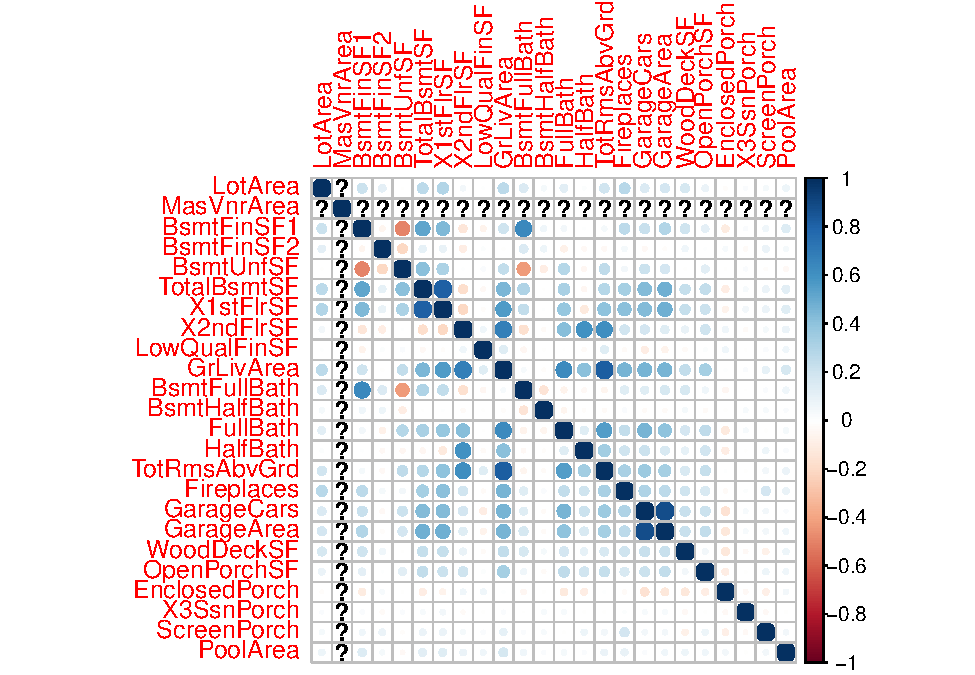
\includegraphics{ScriptJose_files/figure-latex/unnamed-chunk-4-1.pdf}

\begin{Shaded}
\begin{Highlighting}[]
\KeywordTok{qqnorm}\NormalTok{(}\KeywordTok{na.omit}\NormalTok{(}\KeywordTok{as.numeric}\NormalTok{(dataSet}\OperatorTok{$}\NormalTok{BsmtFinSF1)),}\DataTypeTok{main =} \StringTok{"Distribucion normal de BsmtFinSF1"}\NormalTok{)}
\KeywordTok{qqline}\NormalTok{(}\KeywordTok{na.omit}\NormalTok{(}\KeywordTok{as.numeric}\NormalTok{(dataSet}\OperatorTok{$}\NormalTok{BsmtFinSF1)))}
\end{Highlighting}
\end{Shaded}

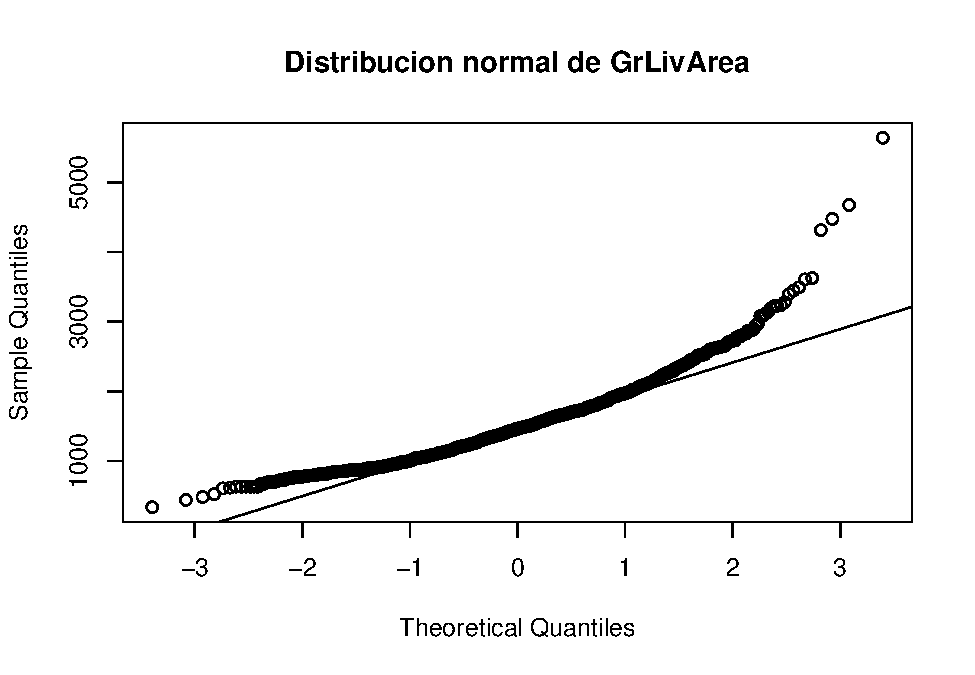
\includegraphics{ScriptJose_files/figure-latex/unnamed-chunk-5-1.pdf}

\begin{Shaded}
\begin{Highlighting}[]
\KeywordTok{qqnorm}\NormalTok{(}\KeywordTok{na.omit}\NormalTok{(}\KeywordTok{as.numeric}\NormalTok{(dataSet}\OperatorTok{$}\NormalTok{WoodDeckSF)),}\DataTypeTok{main =} \StringTok{"Distribucion normal de WoodDeckSF"}\NormalTok{)}
\KeywordTok{qqline}\NormalTok{(}\KeywordTok{na.omit}\NormalTok{(}\KeywordTok{as.numeric}\NormalTok{(dataSet}\OperatorTok{$}\NormalTok{WoodDeckSF)))}
\end{Highlighting}
\end{Shaded}

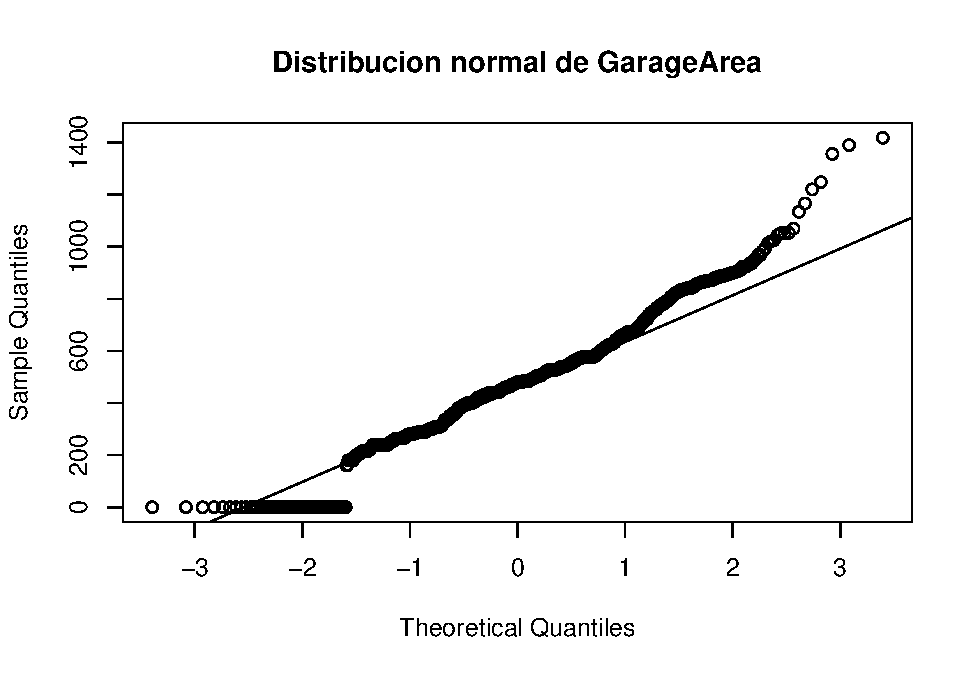
\includegraphics{ScriptJose_files/figure-latex/unnamed-chunk-6-1.pdf}

\begin{Shaded}
\begin{Highlighting}[]
\KeywordTok{qqnorm}\NormalTok{(}\KeywordTok{na.omit}\NormalTok{(}\KeywordTok{as.numeric}\NormalTok{(dataSet}\OperatorTok{$}\NormalTok{X2ndFlrSF)),}\DataTypeTok{main =} \StringTok{"Distribucion normal de X2ndFlrSF"}\NormalTok{)}
\KeywordTok{qqline}\NormalTok{(}\KeywordTok{na.omit}\NormalTok{(}\KeywordTok{as.numeric}\NormalTok{(dataSet}\OperatorTok{$}\NormalTok{X2ndFlrSF)))}
\end{Highlighting}
\end{Shaded}

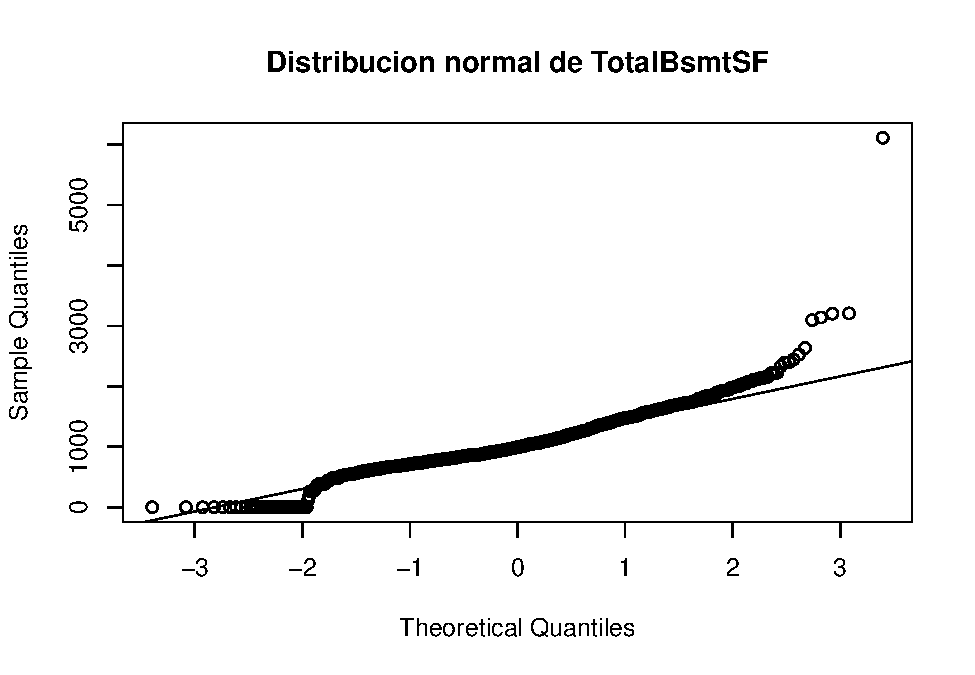
\includegraphics{ScriptJose_files/figure-latex/unnamed-chunk-7-1.pdf}

\begin{Shaded}
\begin{Highlighting}[]
\KeywordTok{qqnorm}\NormalTok{(}\KeywordTok{na.omit}\NormalTok{(}\KeywordTok{as.numeric}\NormalTok{(dataSet}\OperatorTok{$}\NormalTok{OpenPorchSF)),}\DataTypeTok{main =} \StringTok{"Distribucion normal de OpenPorchSF"}\NormalTok{)}
\KeywordTok{qqline}\NormalTok{(}\KeywordTok{na.omit}\NormalTok{(}\KeywordTok{as.numeric}\NormalTok{(dataSet}\OperatorTok{$}\NormalTok{OpenPorchSF)))}
\end{Highlighting}
\end{Shaded}

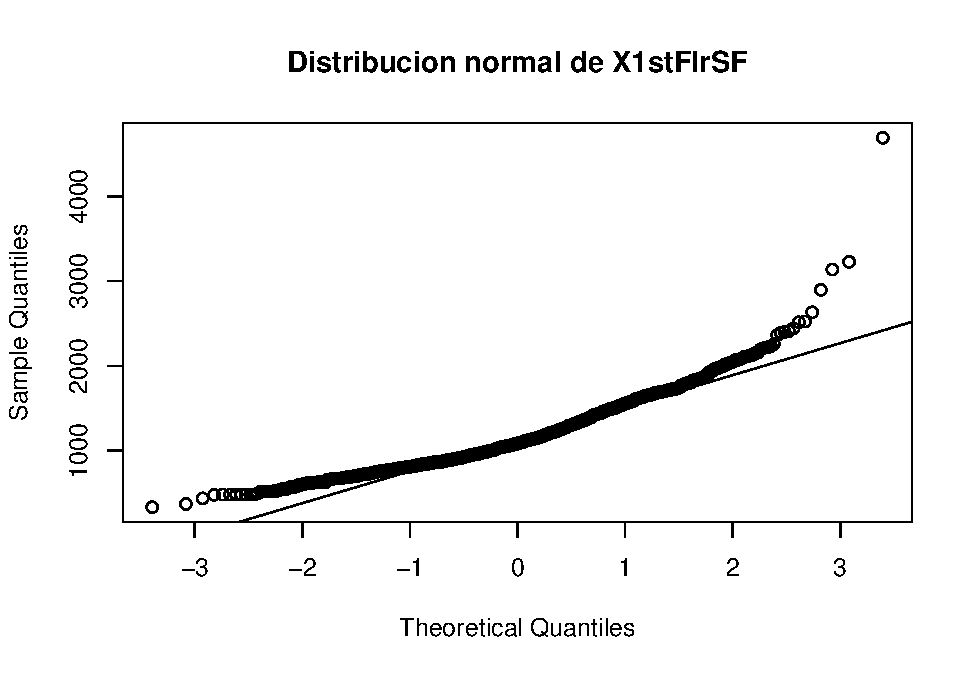
\includegraphics{ScriptJose_files/figure-latex/unnamed-chunk-8-1.pdf}

\begin{Shaded}
\begin{Highlighting}[]
\KeywordTok{qqnorm}\NormalTok{(}\KeywordTok{na.omit}\NormalTok{(}\KeywordTok{as.numeric}\NormalTok{(dataSet}\OperatorTok{$}\NormalTok{LotArea)),}\DataTypeTok{main =} \StringTok{"Distribucion normal de LotArea"}\NormalTok{)}
\KeywordTok{qqline}\NormalTok{(}\KeywordTok{na.omit}\NormalTok{(}\KeywordTok{as.numeric}\NormalTok{(dataSet}\OperatorTok{$}\NormalTok{LotArea)))}
\end{Highlighting}
\end{Shaded}

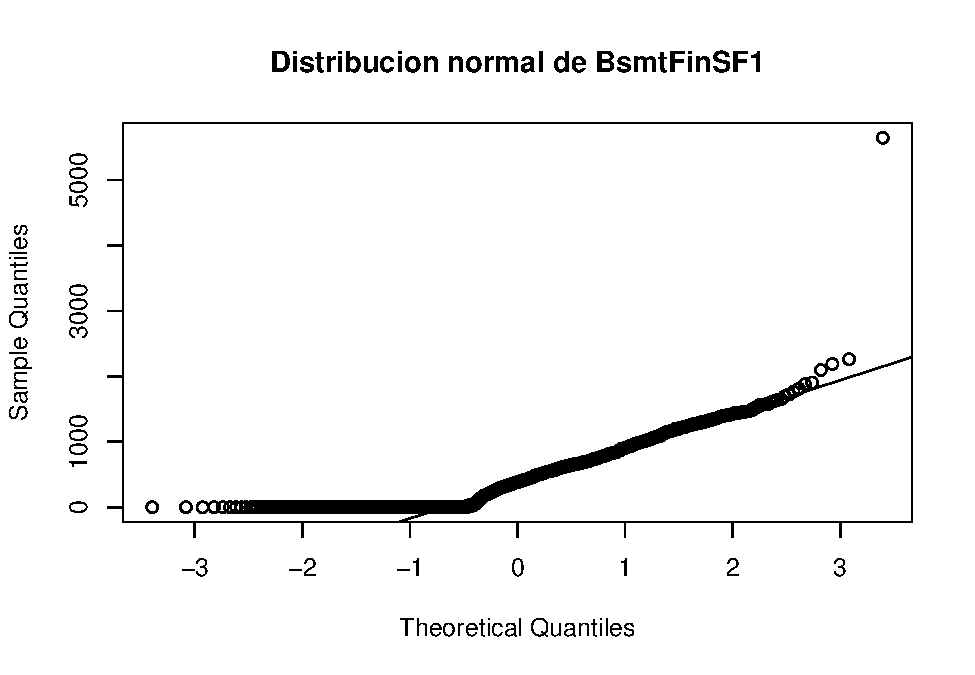
\includegraphics{ScriptJose_files/figure-latex/unnamed-chunk-9-1.pdf}

\begin{Shaded}
\begin{Highlighting}[]
\KeywordTok{qqnorm}\NormalTok{(}\KeywordTok{na.omit}\NormalTok{(}\KeywordTok{as.numeric}\NormalTok{(dataSet}\OperatorTok{$}\NormalTok{BsmtUnfSF)),}\DataTypeTok{main =} \StringTok{"Distribucion normal de BsmtUnfSF"}\NormalTok{)}
\KeywordTok{qqline}\NormalTok{(}\KeywordTok{na.omit}\NormalTok{(}\KeywordTok{as.numeric}\NormalTok{(dataSet}\OperatorTok{$}\NormalTok{BsmtUnfSF)))}
\end{Highlighting}
\end{Shaded}

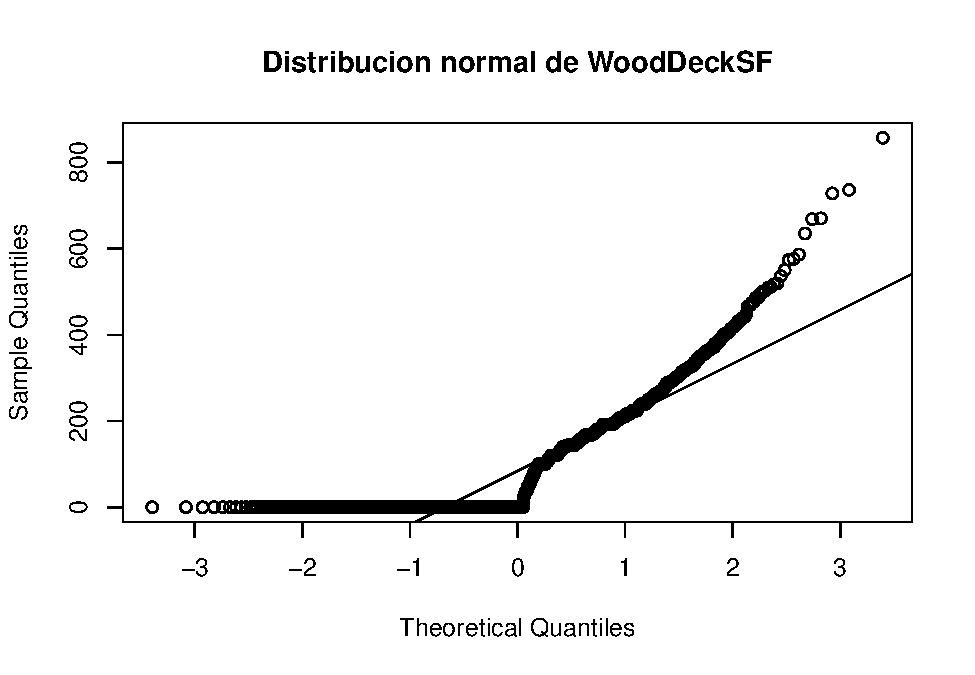
\includegraphics{ScriptJose_files/figure-latex/unnamed-chunk-10-1.pdf}

\begin{Shaded}
\begin{Highlighting}[]
\KeywordTok{qqnorm}\NormalTok{(}\KeywordTok{na.omit}\NormalTok{(}\KeywordTok{as.numeric}\NormalTok{(dataSet}\OperatorTok{$}\NormalTok{ScreenPorch)),}\DataTypeTok{main =} \StringTok{"Distribucion normal de ScreenPorch"}\NormalTok{)}
\KeywordTok{qqline}\NormalTok{(}\KeywordTok{na.omit}\NormalTok{(}\KeywordTok{as.numeric}\NormalTok{(dataSet}\OperatorTok{$}\NormalTok{ScreenPorch)))}
\end{Highlighting}
\end{Shaded}

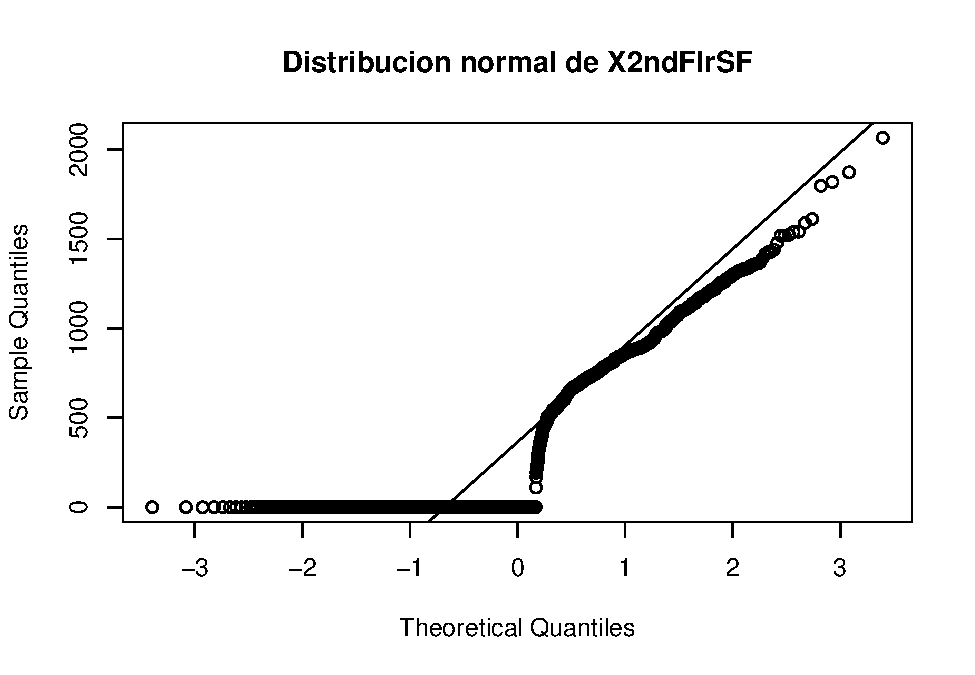
\includegraphics{ScriptJose_files/figure-latex/unnamed-chunk-11-1.pdf}

\begin{Shaded}
\begin{Highlighting}[]
\KeywordTok{qqnorm}\NormalTok{(}\KeywordTok{na.omit}\NormalTok{(}\KeywordTok{as.numeric}\NormalTok{(dataSet}\OperatorTok{$}\NormalTok{PoolArea)),}\DataTypeTok{main =} \StringTok{"Distribucion normal de PoolArea"}\NormalTok{)}
\KeywordTok{qqline}\NormalTok{(}\KeywordTok{na.omit}\NormalTok{(}\KeywordTok{as.numeric}\NormalTok{(dataSet}\OperatorTok{$}\NormalTok{PoolArea)))}
\end{Highlighting}
\end{Shaded}

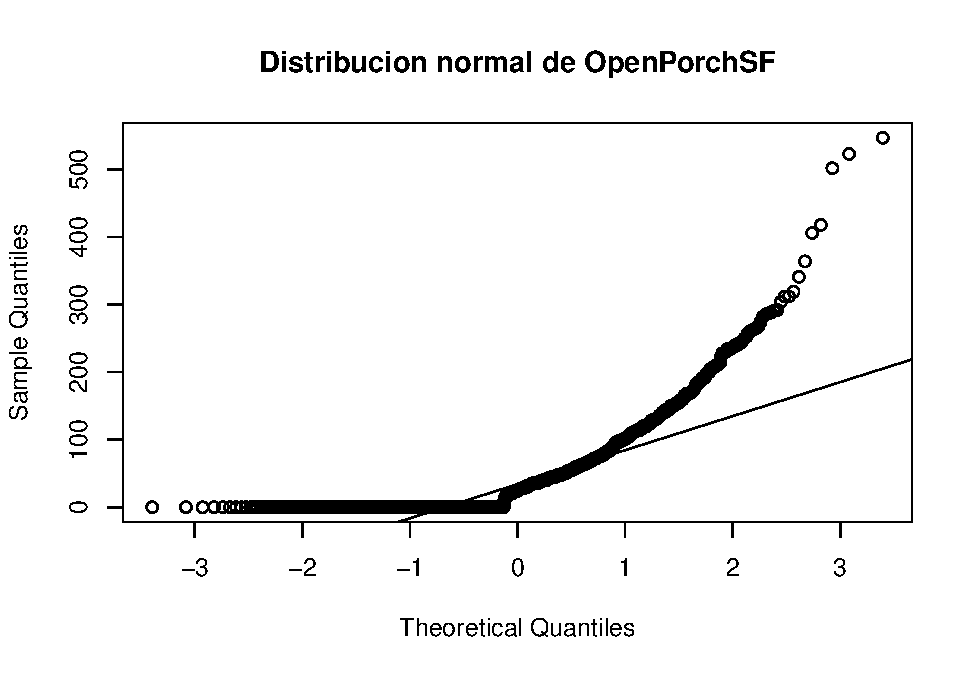
\includegraphics{ScriptJose_files/figure-latex/unnamed-chunk-12-1.pdf}

\begin{Shaded}
\begin{Highlighting}[]
\KeywordTok{qqnorm}\NormalTok{(}\KeywordTok{na.omit}\NormalTok{(}\KeywordTok{as.numeric}\NormalTok{(dataSet}\OperatorTok{$}\NormalTok{X3SsnPorch)),}\DataTypeTok{main =} \StringTok{"Distribucion normal de X3SsnPorch"}\NormalTok{)}
\KeywordTok{qqline}\NormalTok{(}\KeywordTok{na.omit}\NormalTok{(}\KeywordTok{as.numeric}\NormalTok{(dataSet}\OperatorTok{$}\NormalTok{X3SsnPorch)))}
\end{Highlighting}
\end{Shaded}

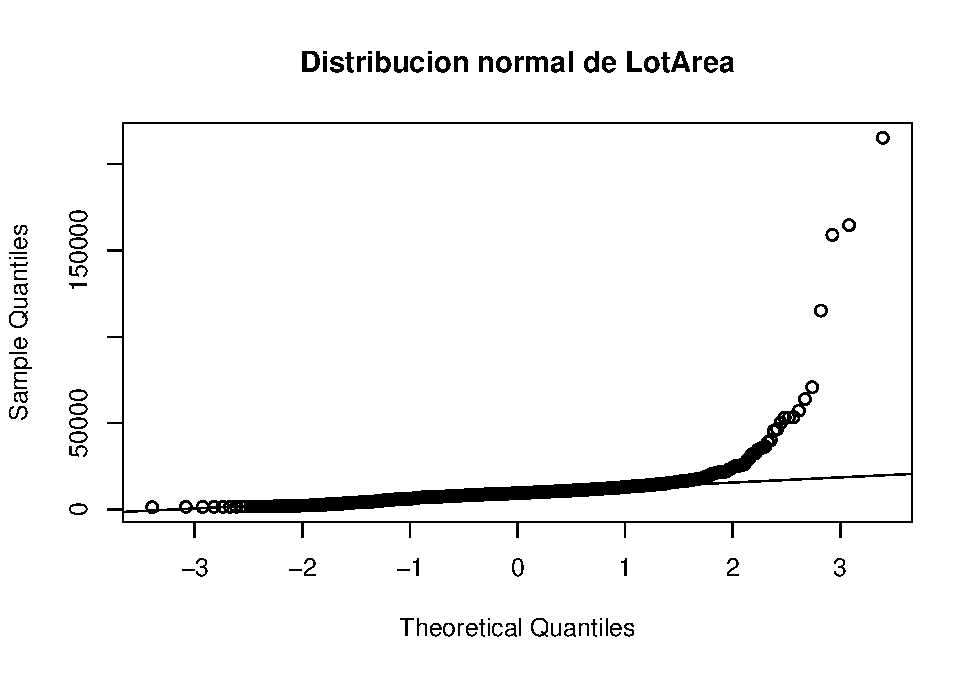
\includegraphics{ScriptJose_files/figure-latex/unnamed-chunk-13-1.pdf}

\begin{Shaded}
\begin{Highlighting}[]
\KeywordTok{qqnorm}\NormalTok{(}\KeywordTok{na.omit}\NormalTok{(}\KeywordTok{as.numeric}\NormalTok{(dataSet}\OperatorTok{$}\NormalTok{BsmtFinSF2)),}\DataTypeTok{main =} \StringTok{"Distribucion normal de BsmtFinSF2"}\NormalTok{)}
\KeywordTok{qqline}\NormalTok{(}\KeywordTok{na.omit}\NormalTok{(}\KeywordTok{as.numeric}\NormalTok{(dataSet}\OperatorTok{$}\NormalTok{BsmtFinSF2)))}
\end{Highlighting}
\end{Shaded}

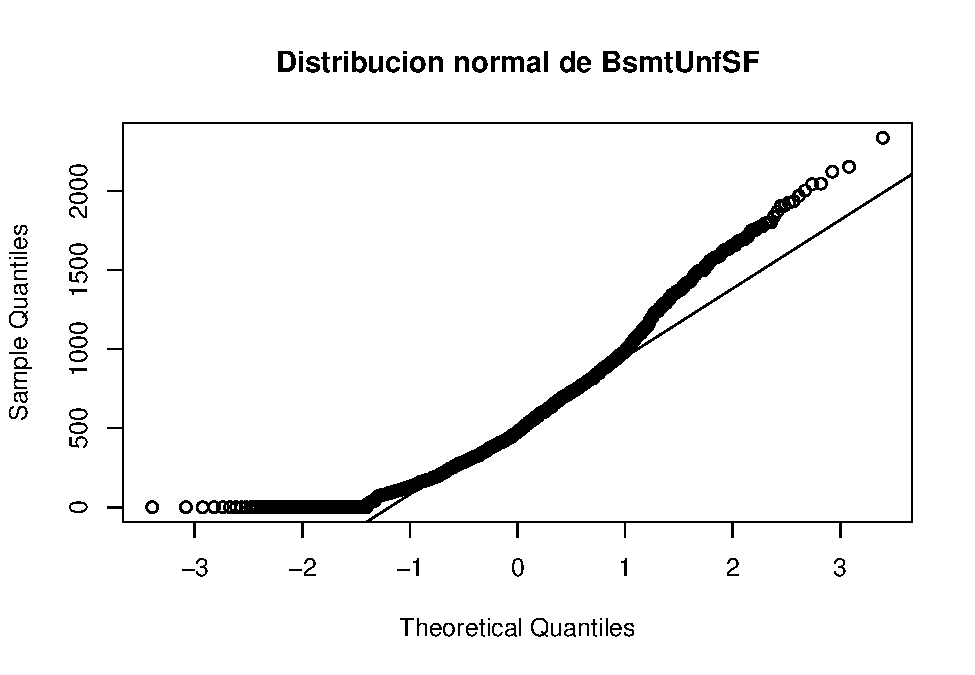
\includegraphics{ScriptJose_files/figure-latex/unnamed-chunk-14-1.pdf}

\begin{Shaded}
\begin{Highlighting}[]
\KeywordTok{qqnorm}\NormalTok{(}\KeywordTok{na.omit}\NormalTok{(}\KeywordTok{as.numeric}\NormalTok{(dataSet}\OperatorTok{$}\NormalTok{BsmtHalfBath)),}\DataTypeTok{main =} \StringTok{"Distribucion normal de BsmtHalfBath"}\NormalTok{)}
\KeywordTok{qqline}\NormalTok{(}\KeywordTok{na.omit}\NormalTok{(}\KeywordTok{as.numeric}\NormalTok{(dataSet}\OperatorTok{$}\NormalTok{BsmtHalfBath)))}
\end{Highlighting}
\end{Shaded}

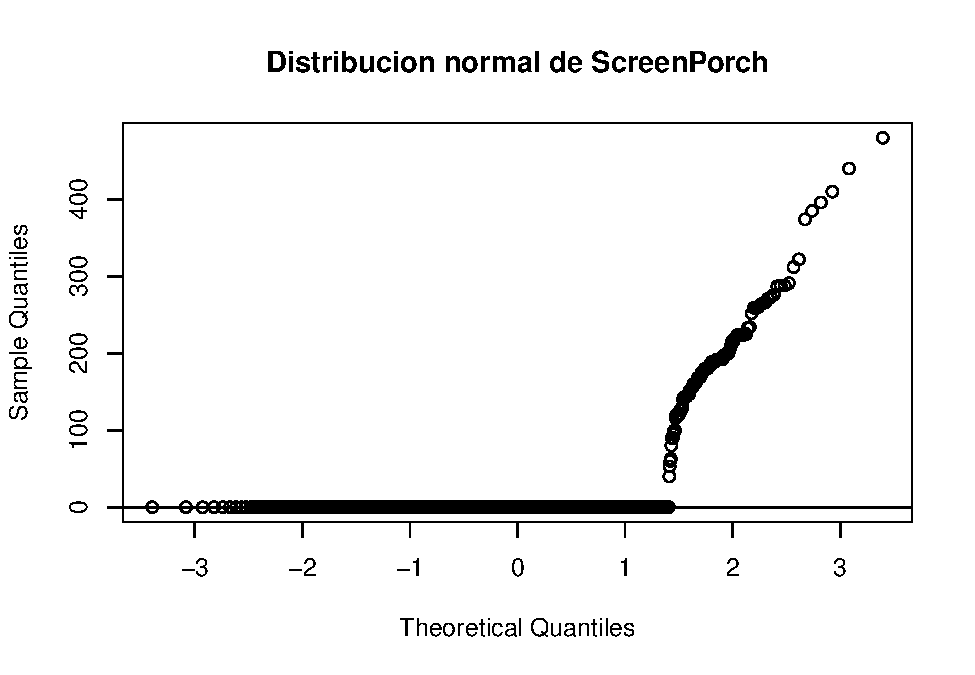
\includegraphics{ScriptJose_files/figure-latex/unnamed-chunk-15-1.pdf}

\begin{Shaded}
\begin{Highlighting}[]
\KeywordTok{qqnorm}\NormalTok{(}\KeywordTok{na.omit}\NormalTok{(}\KeywordTok{as.numeric}\NormalTok{(dataSet}\OperatorTok{$}\NormalTok{LowQualFinSF)),}\DataTypeTok{main =} \StringTok{"Distribucion normal de LowQualFinSF"}\NormalTok{)}
\KeywordTok{qqline}\NormalTok{(}\KeywordTok{na.omit}\NormalTok{(}\KeywordTok{as.numeric}\NormalTok{(dataSet}\OperatorTok{$}\NormalTok{LowQualFinSF)))}
\end{Highlighting}
\end{Shaded}

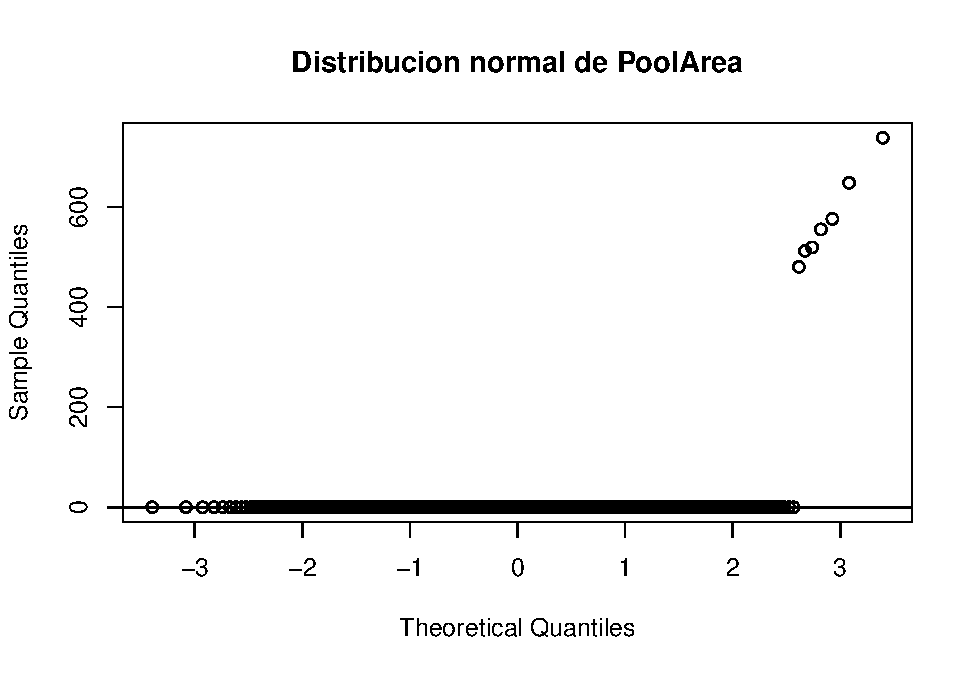
\includegraphics{ScriptJose_files/figure-latex/unnamed-chunk-16-1.pdf}

\begin{Shaded}
\begin{Highlighting}[]
\KeywordTok{qqnorm}\NormalTok{(}\KeywordTok{na.omit}\NormalTok{(}\KeywordTok{as.numeric}\NormalTok{(dataSet}\OperatorTok{$}\NormalTok{KitchenAbvGr)),}\DataTypeTok{main =} \StringTok{"Distribucion normal de KitchenAbvGr"}\NormalTok{)}
\KeywordTok{qqline}\NormalTok{(}\KeywordTok{na.omit}\NormalTok{(}\KeywordTok{as.numeric}\NormalTok{(dataSet}\OperatorTok{$}\NormalTok{KitchenAbvGr)))}
\end{Highlighting}
\end{Shaded}

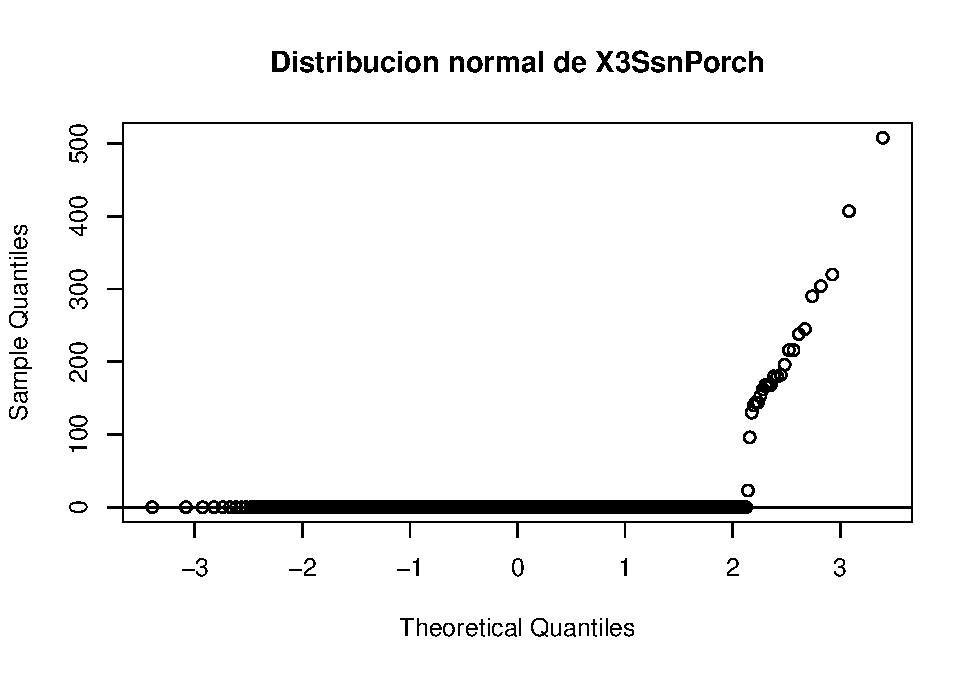
\includegraphics{ScriptJose_files/figure-latex/unnamed-chunk-17-1.pdf}

\begin{verbatim}
## Warning in na.omit(as.numeric(dataSet$LotFrontage)): NAs introducidos por
## coerción

## Warning in na.omit(as.numeric(dataSet$LotFrontage)): NAs introducidos por
## coerción
\end{verbatim}

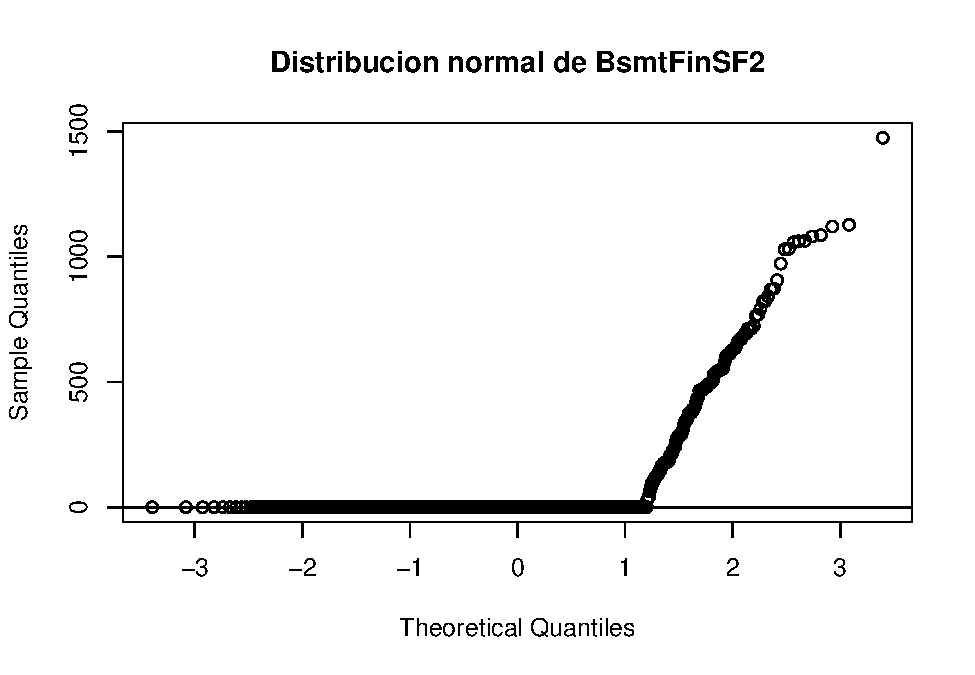
\includegraphics{ScriptJose_files/figure-latex/unnamed-chunk-18-1.pdf}

\begin{verbatim}
## Warning in na.omit(as.numeric(dataSet$MasVnrArea)): NAs introducidos por
## coerción

## Warning in na.omit(as.numeric(dataSet$MasVnrArea)): NAs introducidos por
## coerción
\end{verbatim}

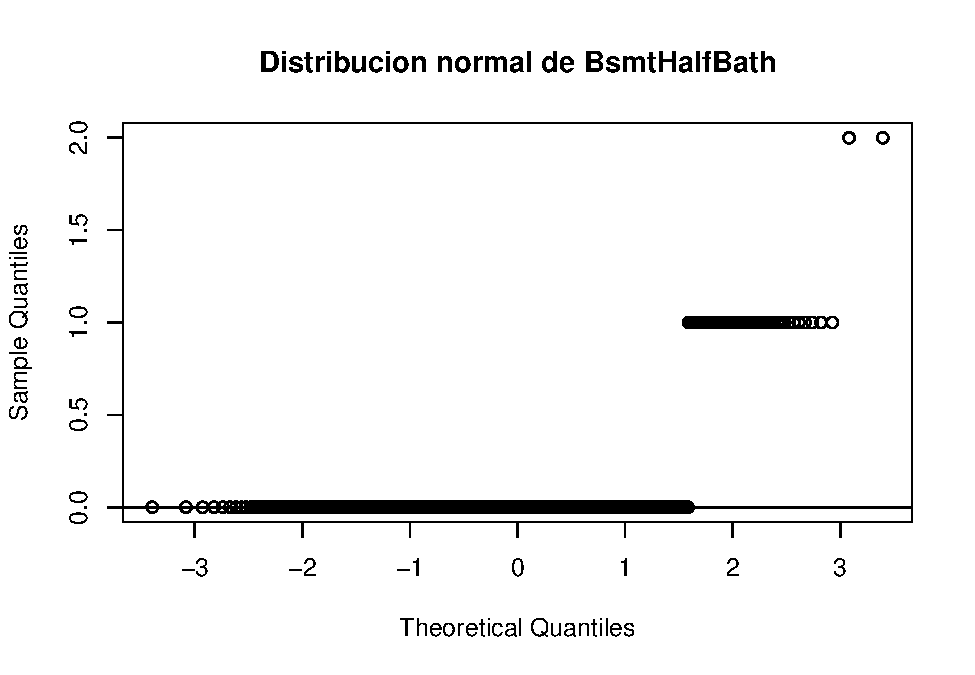
\includegraphics{ScriptJose_files/figure-latex/unnamed-chunk-19-1.pdf}

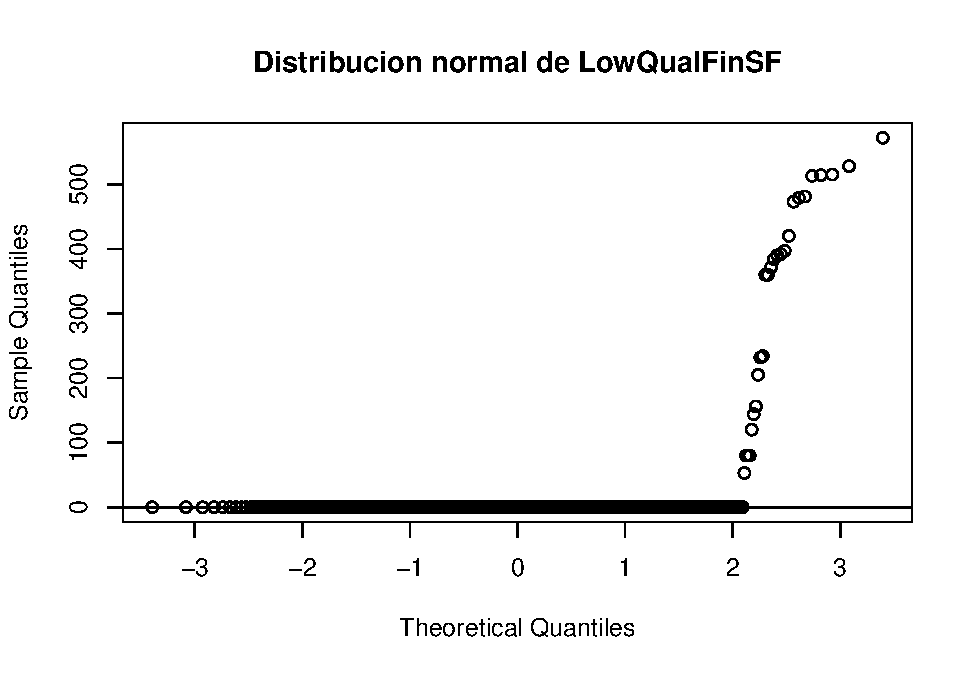
\includegraphics{ScriptJose_files/figure-latex/unnamed-chunk-20-1.pdf}

\hypertarget{anuxe1lisis-de-variables-cualitativas}{%
\section{Análisis de variables
cualitativas}\label{anuxe1lisis-de-variables-cualitativas}}

\hypertarget{tablas-de-frecuencia-y-gruxe1ficas-de-distribuciuxf3n}{%
\subsubsection{Tablas de frecuencia y gráficas de
distribución}\label{tablas-de-frecuencia-y-gruxe1ficas-de-distribuciuxf3n}}

A continuación,

\begin{Shaded}
\begin{Highlighting}[]
\KeywordTok{barplot}\NormalTok{(}\KeywordTok{table}\NormalTok{(dataSet}\OperatorTok{$}\NormalTok{MSZoning),}\DataTypeTok{main =} \StringTok{"Distribución MSZoning"}\NormalTok{,}
        \DataTypeTok{xlab=}\StringTok{"MSZoning"}\NormalTok{)}
\end{Highlighting}
\end{Shaded}

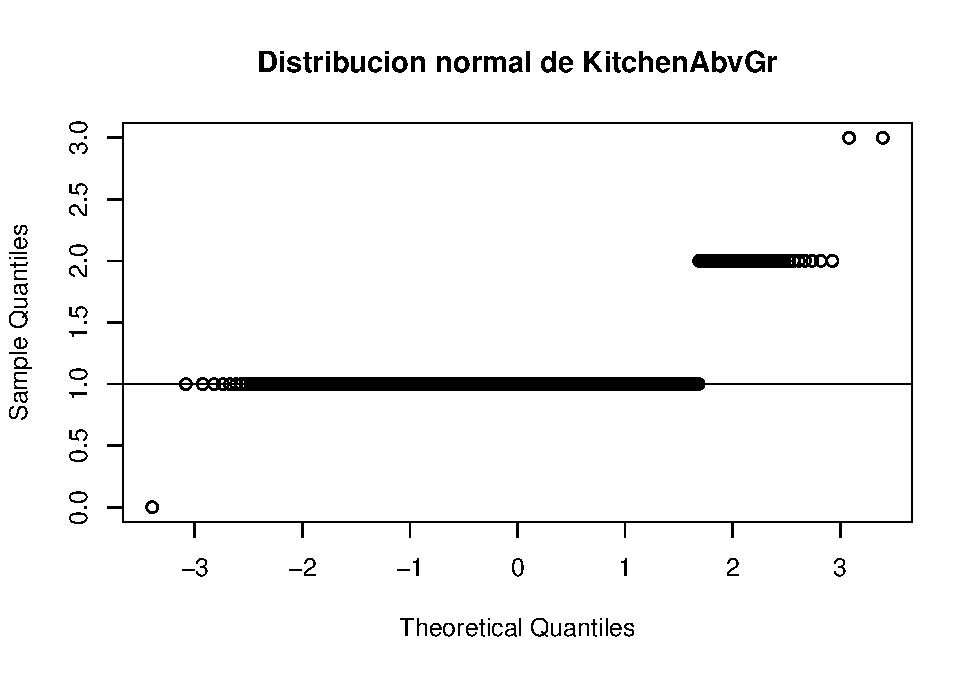
\includegraphics{ScriptJose_files/figure-latex/unnamed-chunk-21-1.pdf}

\begin{Shaded}
\begin{Highlighting}[]
\KeywordTok{barplot}\NormalTok{(}\KeywordTok{table}\NormalTok{(dataSet}\OperatorTok{$}\NormalTok{MSSubClass),}\DataTypeTok{main =} \StringTok{"Distribución MSSubClass"}\NormalTok{,}
        \DataTypeTok{xlab=}\StringTok{"MSSubClass"}\NormalTok{)}
\end{Highlighting}
\end{Shaded}

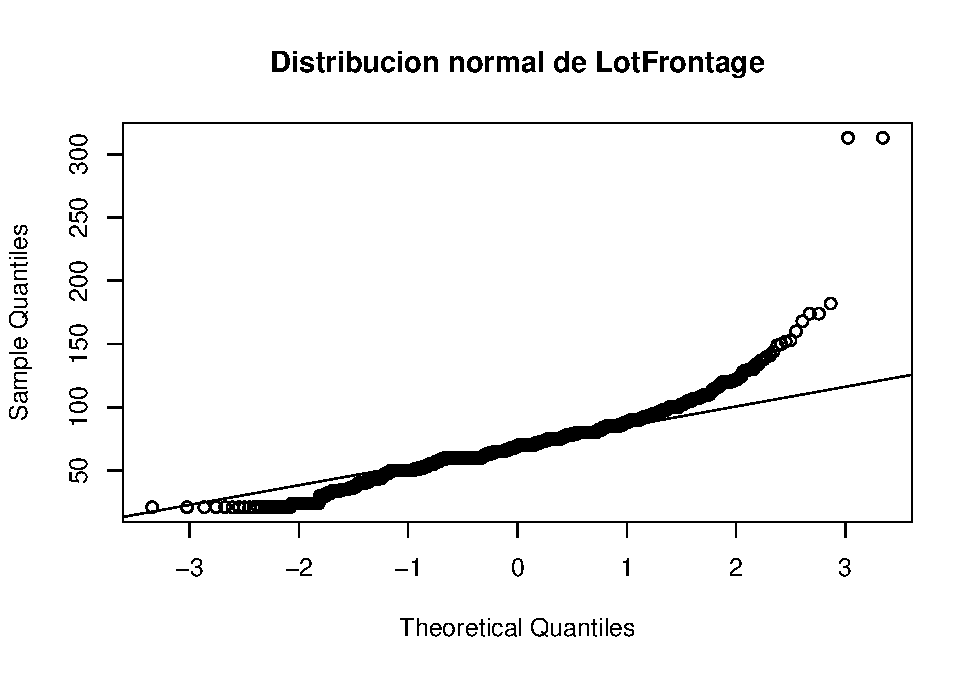
\includegraphics{ScriptJose_files/figure-latex/unnamed-chunk-22-1.pdf}

\begin{Shaded}
\begin{Highlighting}[]
\KeywordTok{barplot}\NormalTok{(}\KeywordTok{table}\NormalTok{(dataSet}\OperatorTok{$}\NormalTok{Street),}\DataTypeTok{main =} \StringTok{"Distribución Street"}\NormalTok{,}
        \DataTypeTok{xlab=}\StringTok{"Street"}\NormalTok{)}
\end{Highlighting}
\end{Shaded}

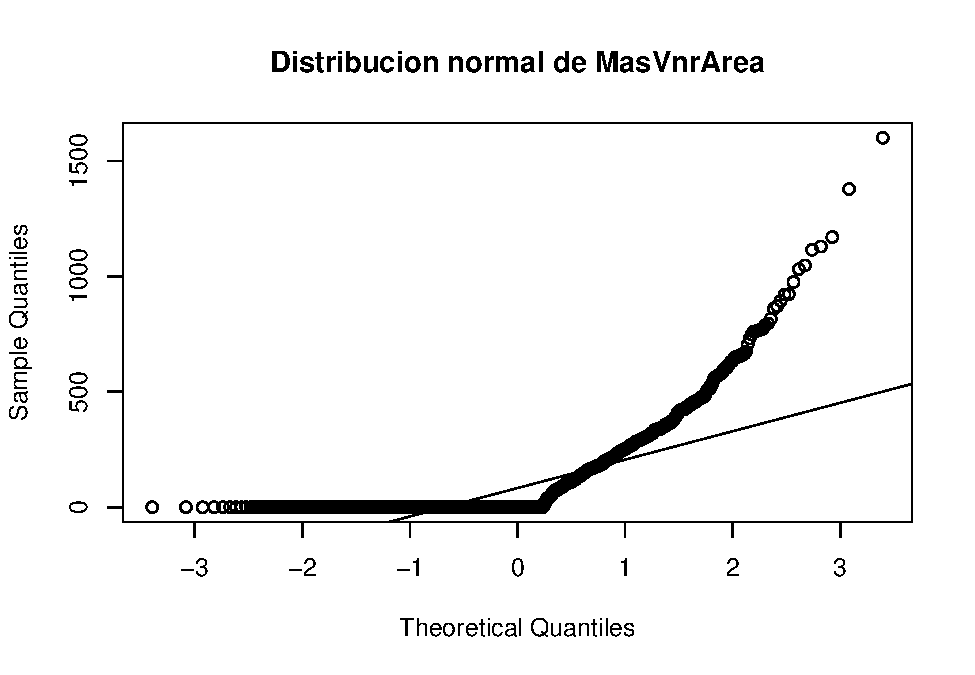
\includegraphics{ScriptJose_files/figure-latex/unnamed-chunk-23-1.pdf}

\begin{Shaded}
\begin{Highlighting}[]
\KeywordTok{barplot}\NormalTok{(}\KeywordTok{table}\NormalTok{(dataSet}\OperatorTok{$}\NormalTok{Alley),}\DataTypeTok{main =} \StringTok{"Distribución Alley"}\NormalTok{,}
        \DataTypeTok{xlab=}\StringTok{"Alley"}\NormalTok{)}
\end{Highlighting}
\end{Shaded}

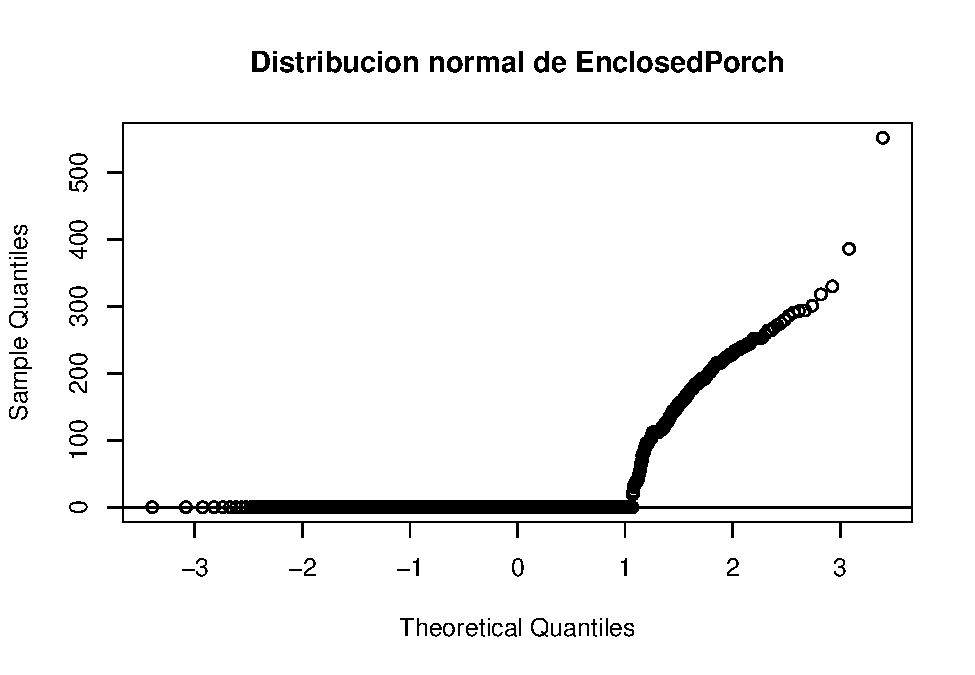
\includegraphics{ScriptJose_files/figure-latex/unnamed-chunk-24-1.pdf}

\begin{Shaded}
\begin{Highlighting}[]
\KeywordTok{barplot}\NormalTok{(}\KeywordTok{table}\NormalTok{(dataSet}\OperatorTok{$}\NormalTok{LotShape),}\DataTypeTok{main =} \StringTok{"Distribución LotShape"}\NormalTok{,}
        \DataTypeTok{xlab=}\StringTok{"LotShape"}\NormalTok{)}
\end{Highlighting}
\end{Shaded}

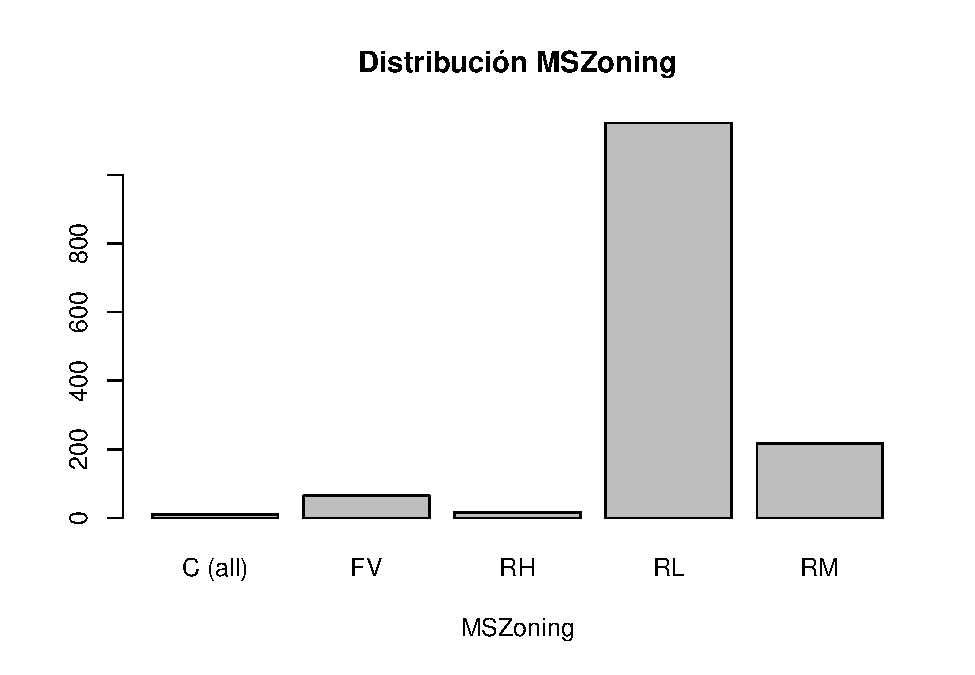
\includegraphics{ScriptJose_files/figure-latex/unnamed-chunk-25-1.pdf}

\begin{Shaded}
\begin{Highlighting}[]
\KeywordTok{barplot}\NormalTok{(}\KeywordTok{table}\NormalTok{(dataSet}\OperatorTok{$}\NormalTok{LandContour),}\DataTypeTok{main =} \StringTok{"Distribución LandContour"}\NormalTok{,}
        \DataTypeTok{xlab=}\StringTok{"LandContour"}\NormalTok{)}
\end{Highlighting}
\end{Shaded}

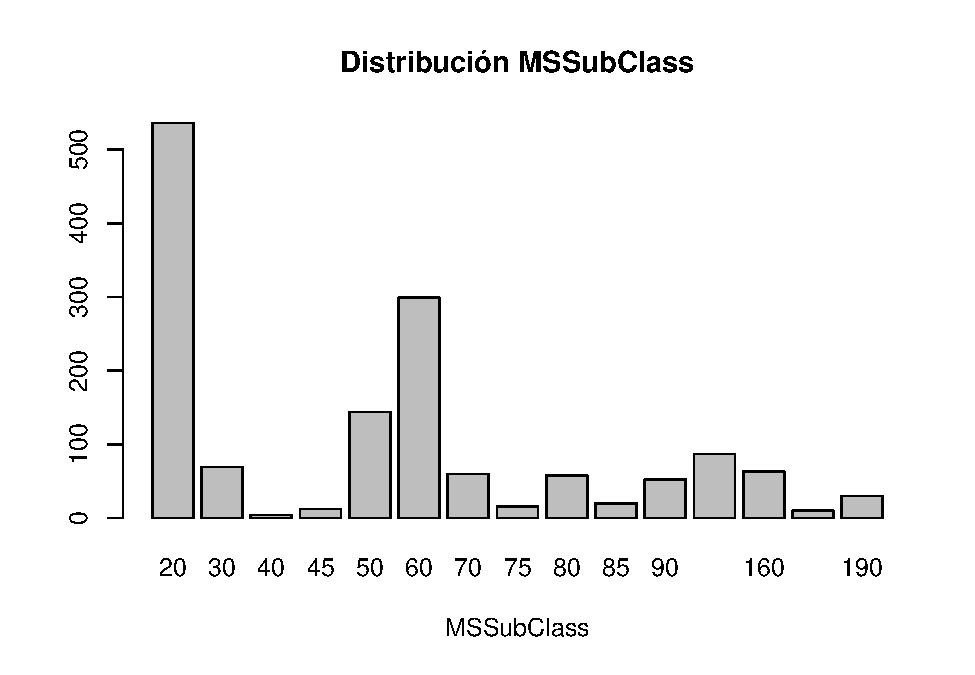
\includegraphics{ScriptJose_files/figure-latex/unnamed-chunk-26-1.pdf}

\begin{Shaded}
\begin{Highlighting}[]
\KeywordTok{barplot}\NormalTok{(}\KeywordTok{table}\NormalTok{(dataSet}\OperatorTok{$}\NormalTok{Utilities),}\DataTypeTok{main =} \StringTok{"Distribución Utilities"}\NormalTok{,}
        \DataTypeTok{xlab=}\StringTok{"Utilities"}\NormalTok{)}
\end{Highlighting}
\end{Shaded}

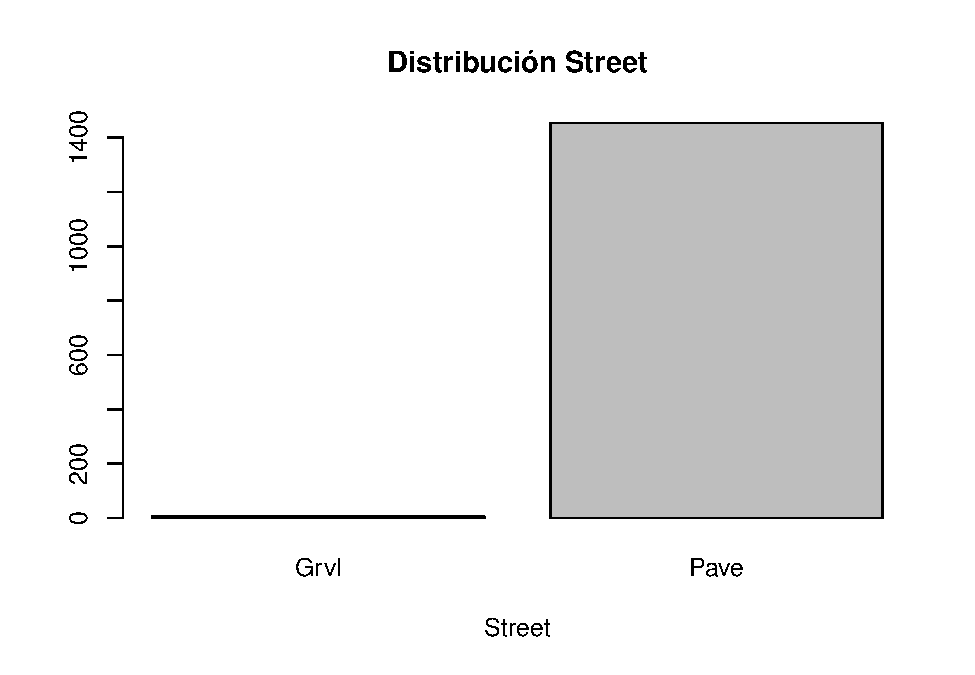
\includegraphics{ScriptJose_files/figure-latex/unnamed-chunk-27-1.pdf}

\begin{Shaded}
\begin{Highlighting}[]
\KeywordTok{barplot}\NormalTok{(}\KeywordTok{table}\NormalTok{(dataSet}\OperatorTok{$}\NormalTok{LotConfig),}\DataTypeTok{main =} \StringTok{"Distribución LotConfig"}\NormalTok{,}
        \DataTypeTok{xlab=}\StringTok{"LotConfig"}\NormalTok{)}
\end{Highlighting}
\end{Shaded}

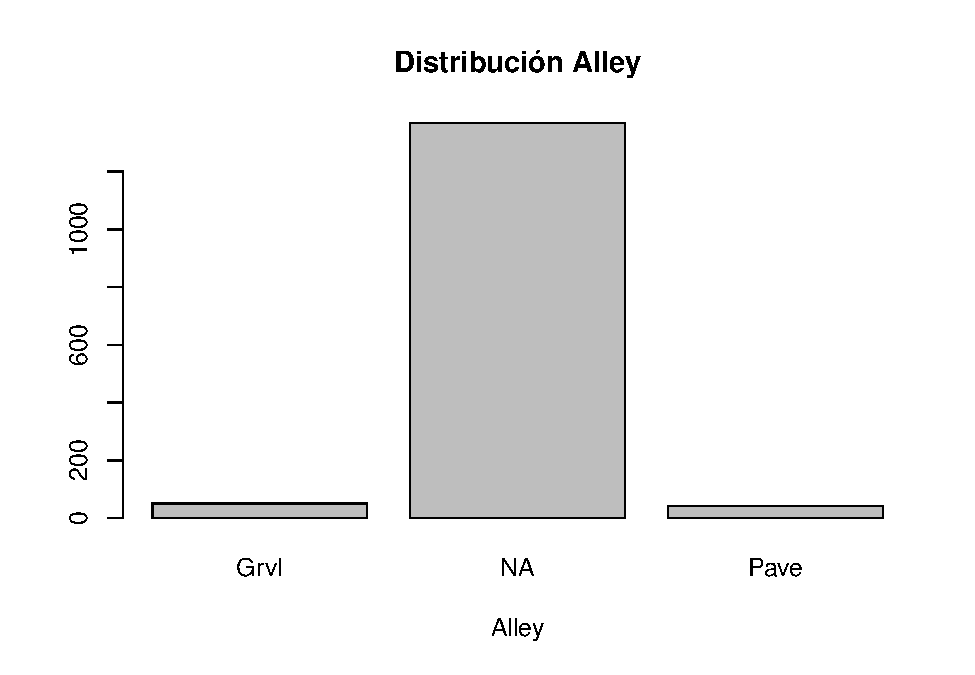
\includegraphics{ScriptJose_files/figure-latex/unnamed-chunk-28-1.pdf}

\begin{Shaded}
\begin{Highlighting}[]
\KeywordTok{barplot}\NormalTok{(}\KeywordTok{table}\NormalTok{(dataSet}\OperatorTok{$}\NormalTok{LandSlope),}\DataTypeTok{main =} \StringTok{"Distribución LandSlope"}\NormalTok{,}
        \DataTypeTok{xlab=}\StringTok{"LandSlope"}\NormalTok{)}
\end{Highlighting}
\end{Shaded}

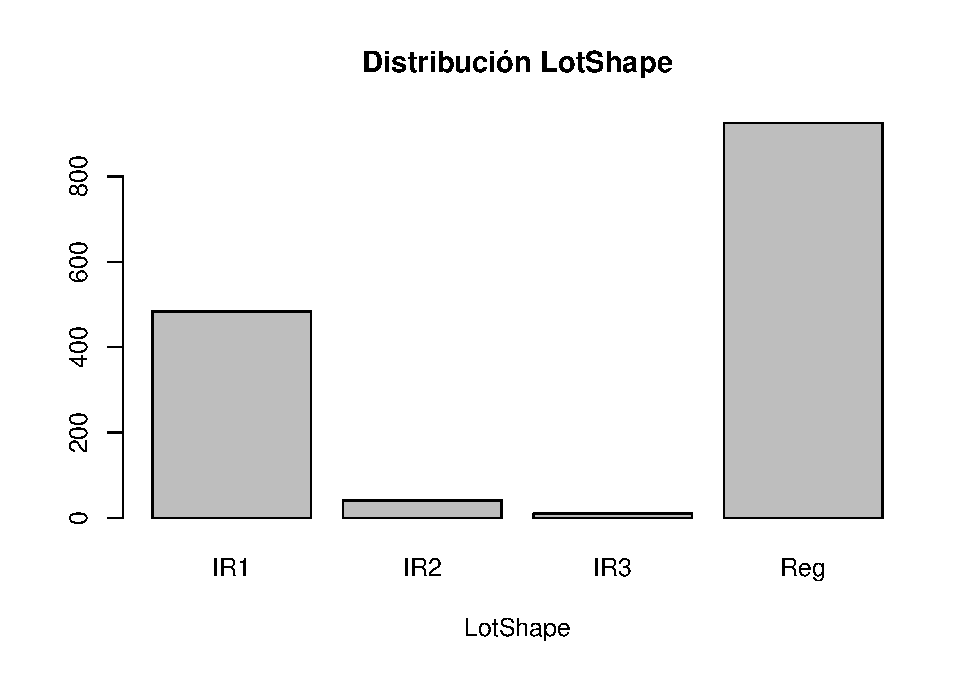
\includegraphics{ScriptJose_files/figure-latex/unnamed-chunk-29-1.pdf}

\begin{Shaded}
\begin{Highlighting}[]
\KeywordTok{barplot}\NormalTok{(}\KeywordTok{table}\NormalTok{(dataSet}\OperatorTok{$}\NormalTok{Neighborhood),}\DataTypeTok{main =} \StringTok{"Distribución Neighborhood"}\NormalTok{,}\DataTypeTok{las=}\DecValTok{2}\NormalTok{)}
\end{Highlighting}
\end{Shaded}

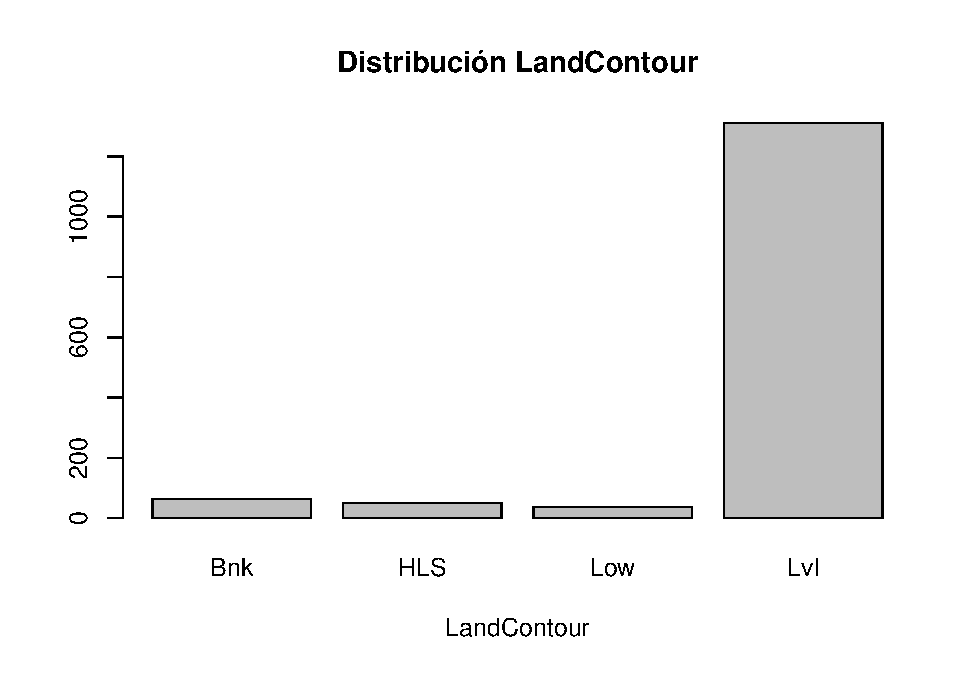
\includegraphics{ScriptJose_files/figure-latex/unnamed-chunk-30-1.pdf}

\begin{Shaded}
\begin{Highlighting}[]
\KeywordTok{barplot}\NormalTok{(}\KeywordTok{table}\NormalTok{(dataSet}\OperatorTok{$}\NormalTok{Condition1),}\DataTypeTok{main =} \StringTok{"Distribución Condition1"}\NormalTok{,}
        \DataTypeTok{xlab=}\StringTok{"Condition1"}\NormalTok{,}\DataTypeTok{las=}\DecValTok{2}\NormalTok{)}
\end{Highlighting}
\end{Shaded}

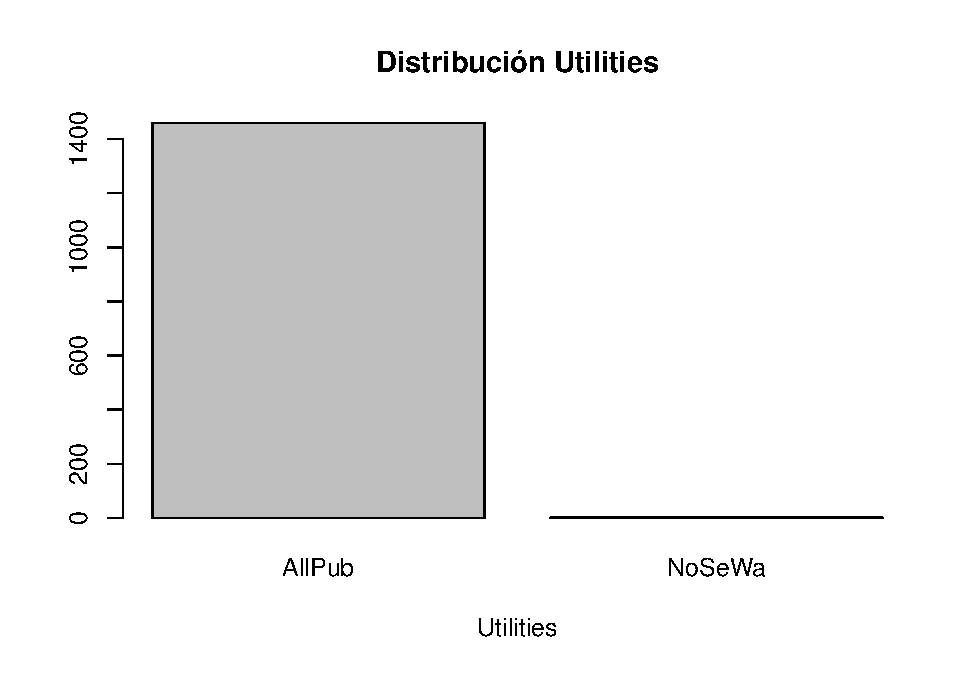
\includegraphics{ScriptJose_files/figure-latex/unnamed-chunk-31-1.pdf}

\begin{Shaded}
\begin{Highlighting}[]
\KeywordTok{barplot}\NormalTok{(}\KeywordTok{table}\NormalTok{(dataSet}\OperatorTok{$}\NormalTok{Condition2),}\DataTypeTok{main =} \StringTok{"Distribución Condition2"}\NormalTok{,}
        \DataTypeTok{xlab=}\StringTok{"Condition2"}\NormalTok{,}\DataTypeTok{las=}\DecValTok{2}\NormalTok{)}
\end{Highlighting}
\end{Shaded}

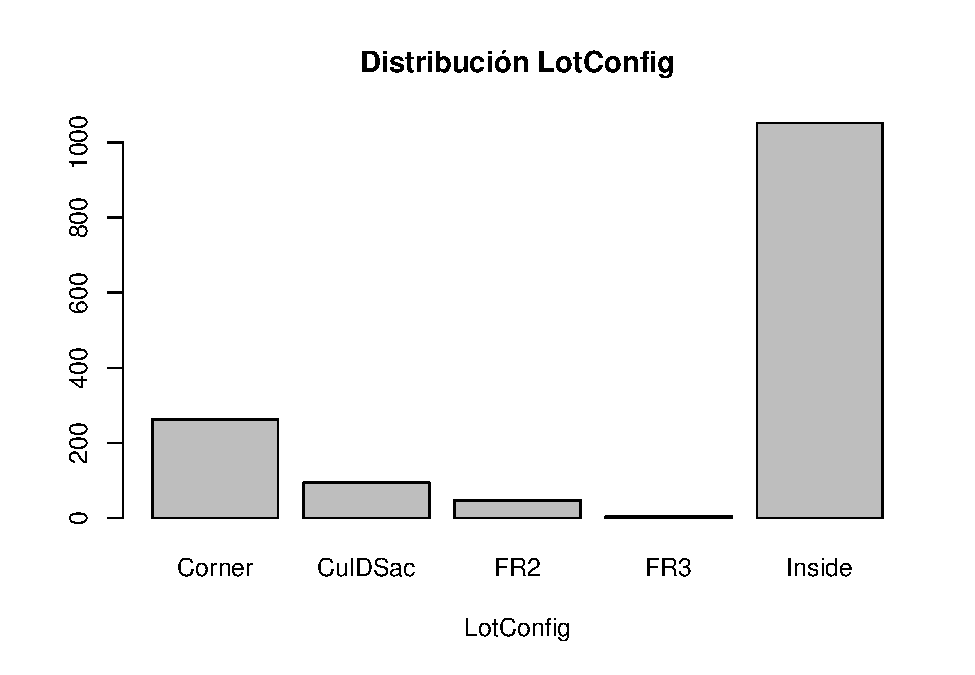
\includegraphics{ScriptJose_files/figure-latex/unnamed-chunk-32-1.pdf}

\begin{Shaded}
\begin{Highlighting}[]
\KeywordTok{barplot}\NormalTok{(}\KeywordTok{table}\NormalTok{(dataSet}\OperatorTok{$}\NormalTok{BldgType),}\DataTypeTok{main =} \StringTok{"Distribución BldgType"}\NormalTok{,}
        \DataTypeTok{xlab=}\StringTok{"BldgType"}\NormalTok{)}
\end{Highlighting}
\end{Shaded}

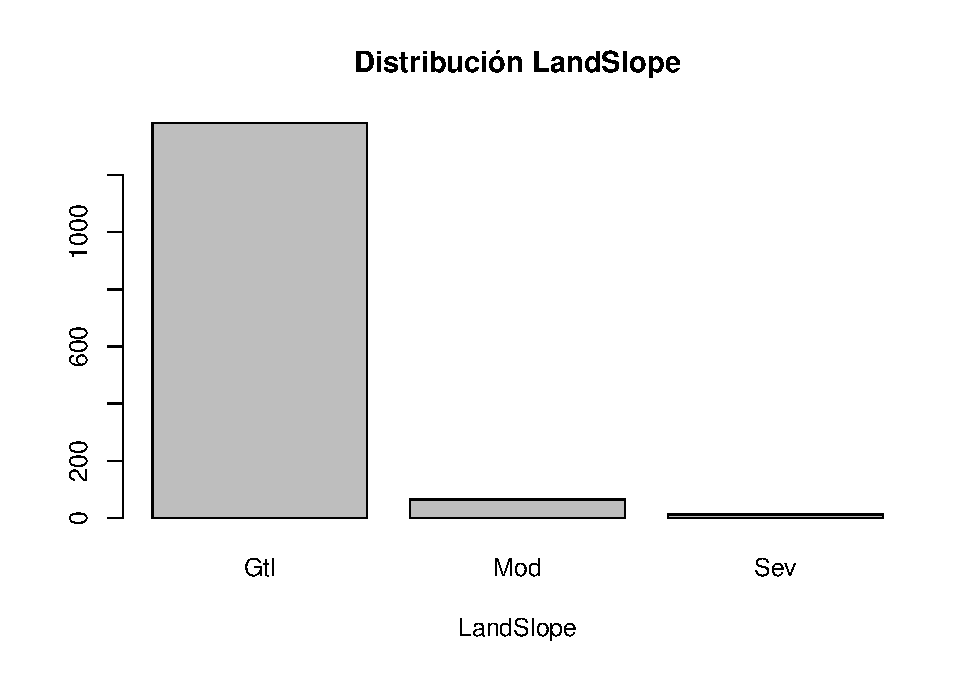
\includegraphics{ScriptJose_files/figure-latex/unnamed-chunk-33-1.pdf}

\begin{Shaded}
\begin{Highlighting}[]
\KeywordTok{barplot}\NormalTok{(}\KeywordTok{table}\NormalTok{(dataSet}\OperatorTok{$}\NormalTok{HouseStyle),}\DataTypeTok{main =} \StringTok{"Distribución HouseStyle"}\NormalTok{,}
        \DataTypeTok{las=}\DecValTok{2}\NormalTok{)}
\end{Highlighting}
\end{Shaded}

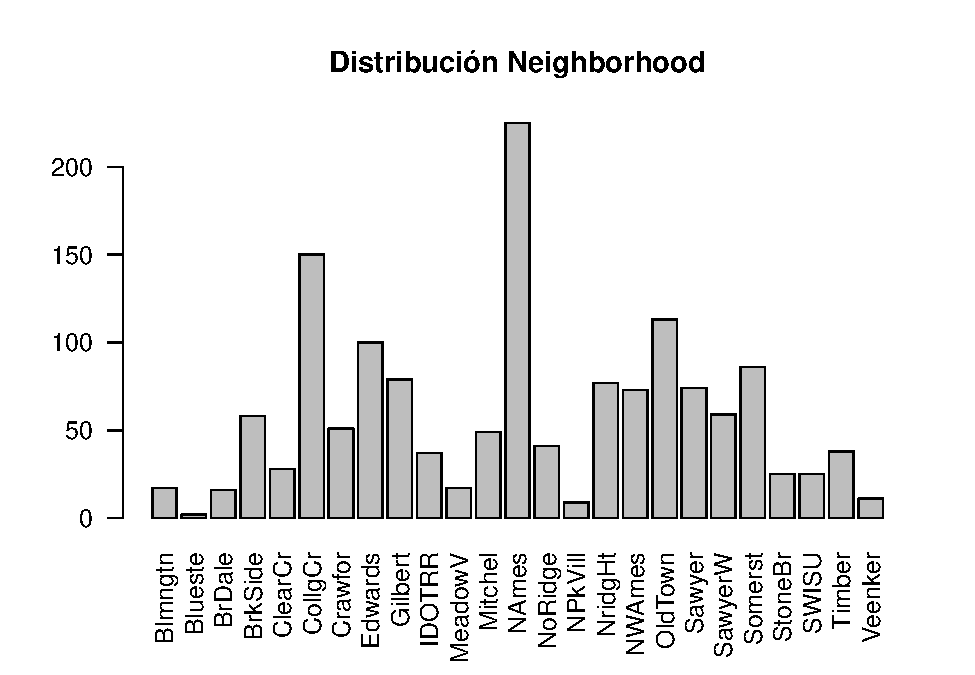
\includegraphics{ScriptJose_files/figure-latex/unnamed-chunk-34-1.pdf}

\begin{Shaded}
\begin{Highlighting}[]
\KeywordTok{barplot}\NormalTok{(}\KeywordTok{table}\NormalTok{(dataSet}\OperatorTok{$}\NormalTok{OverallQual),}\DataTypeTok{main =} \StringTok{"Distribución OverallQual"}\NormalTok{,}
        \DataTypeTok{xlab=}\StringTok{"OverallQual"}\NormalTok{)}
\end{Highlighting}
\end{Shaded}

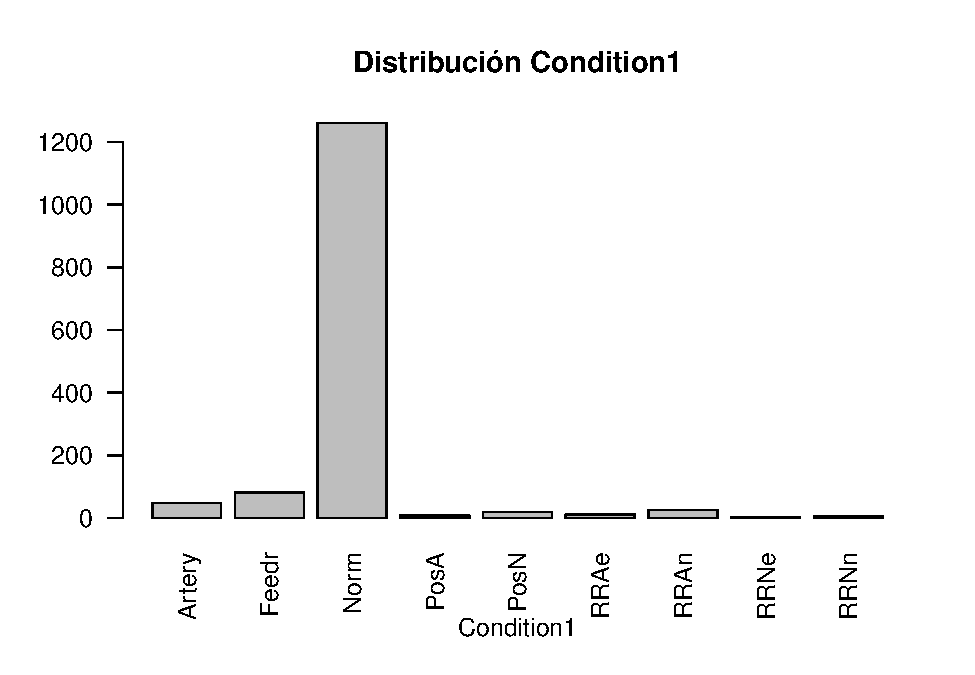
\includegraphics{ScriptJose_files/figure-latex/unnamed-chunk-35-1.pdf}

\begin{Shaded}
\begin{Highlighting}[]
\KeywordTok{barplot}\NormalTok{(}\KeywordTok{table}\NormalTok{(dataSet}\OperatorTok{$}\NormalTok{OverallCond),}\DataTypeTok{main =} \StringTok{"Distribución OverallCond"}\NormalTok{,}
        \DataTypeTok{xlab=}\StringTok{"OverallCond"}\NormalTok{)}
\end{Highlighting}
\end{Shaded}

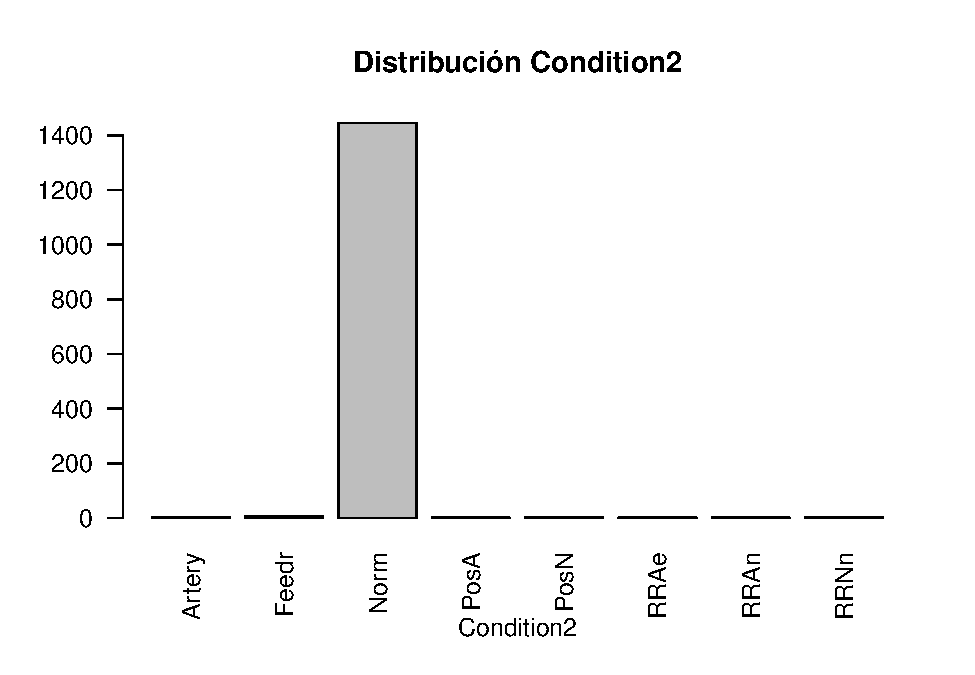
\includegraphics{ScriptJose_files/figure-latex/unnamed-chunk-36-1.pdf}

\begin{Shaded}
\begin{Highlighting}[]
\NormalTok{knitr}\OperatorTok{::}\KeywordTok{kable}\NormalTok{(}
  \KeywordTok{table}\NormalTok{(dataSet}\OperatorTok{$}\NormalTok{YearBuilt), }\DataTypeTok{caption =} \StringTok{'Tabla de frecuencia YearBuilt'}
\NormalTok{)}
\end{Highlighting}
\end{Shaded}

\begin{longtable}[]{@{}lr@{}}
\caption{Tabla de frecuencia YearBuilt}\tabularnewline
\toprule
Var1 & Freq\tabularnewline
\midrule
\endfirsthead
\toprule
Var1 & Freq\tabularnewline
\midrule
\endhead
1872 & 1\tabularnewline
1875 & 1\tabularnewline
1880 & 4\tabularnewline
1882 & 1\tabularnewline
1885 & 2\tabularnewline
1890 & 2\tabularnewline
1892 & 2\tabularnewline
1893 & 1\tabularnewline
1898 & 1\tabularnewline
1900 & 10\tabularnewline
1904 & 1\tabularnewline
1905 & 1\tabularnewline
1906 & 1\tabularnewline
1908 & 2\tabularnewline
1910 & 17\tabularnewline
1911 & 1\tabularnewline
1912 & 3\tabularnewline
1913 & 1\tabularnewline
1914 & 7\tabularnewline
1915 & 10\tabularnewline
1916 & 8\tabularnewline
1917 & 1\tabularnewline
1918 & 7\tabularnewline
1919 & 3\tabularnewline
1920 & 30\tabularnewline
1921 & 6\tabularnewline
1922 & 8\tabularnewline
1923 & 7\tabularnewline
1924 & 7\tabularnewline
1925 & 16\tabularnewline
1926 & 9\tabularnewline
1927 & 3\tabularnewline
1928 & 7\tabularnewline
1929 & 4\tabularnewline
1930 & 9\tabularnewline
1931 & 6\tabularnewline
1932 & 4\tabularnewline
1934 & 3\tabularnewline
1935 & 6\tabularnewline
1936 & 9\tabularnewline
1937 & 5\tabularnewline
1938 & 4\tabularnewline
1939 & 8\tabularnewline
1940 & 18\tabularnewline
1941 & 15\tabularnewline
1942 & 2\tabularnewline
1945 & 6\tabularnewline
1946 & 7\tabularnewline
1947 & 5\tabularnewline
1948 & 14\tabularnewline
1949 & 12\tabularnewline
1950 & 20\tabularnewline
1951 & 6\tabularnewline
1952 & 5\tabularnewline
1953 & 12\tabularnewline
1954 & 24\tabularnewline
1955 & 16\tabularnewline
1956 & 14\tabularnewline
1957 & 20\tabularnewline
1958 & 24\tabularnewline
1959 & 26\tabularnewline
1960 & 17\tabularnewline
1961 & 14\tabularnewline
1962 & 19\tabularnewline
1963 & 16\tabularnewline
1964 & 15\tabularnewline
1965 & 24\tabularnewline
1966 & 18\tabularnewline
1967 & 16\tabularnewline
1968 & 22\tabularnewline
1969 & 14\tabularnewline
1970 & 24\tabularnewline
1971 & 22\tabularnewline
1972 & 23\tabularnewline
1973 & 11\tabularnewline
1974 & 10\tabularnewline
1975 & 8\tabularnewline
1976 & 33\tabularnewline
1977 & 32\tabularnewline
1978 & 16\tabularnewline
1979 & 9\tabularnewline
1980 & 10\tabularnewline
1981 & 5\tabularnewline
1982 & 6\tabularnewline
1983 & 4\tabularnewline
1984 & 9\tabularnewline
1985 & 5\tabularnewline
1986 & 5\tabularnewline
1987 & 3\tabularnewline
1988 & 11\tabularnewline
1989 & 3\tabularnewline
1990 & 12\tabularnewline
1991 & 5\tabularnewline
1992 & 13\tabularnewline
1993 & 17\tabularnewline
1994 & 19\tabularnewline
1995 & 18\tabularnewline
1996 & 15\tabularnewline
1997 & 14\tabularnewline
1998 & 25\tabularnewline
1999 & 25\tabularnewline
2000 & 24\tabularnewline
2001 & 20\tabularnewline
2002 & 23\tabularnewline
2003 & 45\tabularnewline
2004 & 54\tabularnewline
2005 & 64\tabularnewline
2006 & 67\tabularnewline
2007 & 49\tabularnewline
2008 & 23\tabularnewline
2009 & 18\tabularnewline
2010 & 1\tabularnewline
\bottomrule
\end{longtable}

\end{document}
